% !TeX spellcheck = en_GB
\documentclass[a4paper,11pt,oneside]{article}

\usepackage[vmargin=0.8in,outer=0.65in,inner=0.8in]{geometry}

\usepackage{newtxtext} % for roman style text and math
\usepackage{newtxmath}

\usepackage{etoolbox} % for defining and using boolean vars
\usepackage{setspace} % for changing line spacing. Using \linespread is not recommended
\usepackage{xspace} % for space after text macros
\usepackage{enumitem} % for changing settings of enumerate and itemize lists
\usepackage{caption,subcaption} % for changing caption settings
\usepackage{graphicx} % to include figures
\usepackage{float} % for modifications to figure position
\usepackage{standalone} % for stanalone tikz pictures
\usepackage{tikz}
\usetikzlibrary{arrows,calc,shapes,positioning,trees,matrix}
\usepackage{amsmath} % for math support
\usepackage{mathtools} % for math support
%\usepackage{upgreek}
\usepackage{accents}
\usepackage{empheq} % for emphasis (boxing etc) around multiple equations
\usepackage{gensymb} % for degree
\usepackage{bm} % for bold math symbols
\usepackage{cancel}
\usepackage{chemformula} % for chemicals
\usepackage{siunitx} % for units
\usepackage{booktabs} % for well spaced tables
%\usepackage{fancyhdr} % for header and footer
\usepackage{epstopdf} % for inserting .eps files as images
\usepackage[
backend=biber,
style=nature,% important, use this style only
citestyle=numeric-comp,
maxbibnames=50,
sorting=none]%important to specify this
{biblatex}
\usepackage{hyperref}
\hypersetup
{
	colorlinks=true,
	linkcolor=black,
	filecolor=black,      
	urlcolor=black,
	citecolor=black,
	pdftitle={APS-2 report},
}

\usepackage[compress,capitalize]{cleveref} % to be loaded after hyperref
% ``capitalize'' to use capital starting letter in reference
% ``compress'' to prevent sorting multiple references and use compressed referencing
\crefname{subsection}{Subsection}{Subsections} % to refer subsections, label them using \label[subsection]{name}
% Assuming that cleveref is loaded using capitalize option

\setlength{\parindent}{2em}
\setlength{\parskip}{0.5em}

\setlist[enumerate]{
	% vertical spacing
	topsep=0em,
	itemsep=0em,
	% horizontal spacing
	labelindent=0em,
	leftmargin=\parindent,
	labelsep=*,
}
\setlist[itemize]{
	% vertical spacing
	topsep=0em,
	itemsep=0em,
	% horizontal spacing
	labelindent=0em,
	leftmargin=\parindent,
	labelsep=*,
}
\captionsetup[figure]{labelfont={sf,bf},textfont={sf}}
\captionsetup[table]{labelfont={sf,bf},textfont={sf}}

%\addbibresource{references-articles.bib}
%\addbibresource{references-books.bib}
%\addbibresource{references-others.bib}

\newcommand{\newword}[1]{\textbf{#1}} % style of text for introducing a new important word or definition
\newcommand{\citear}[1]{\citeauthor{#1} \cite{#1}} % cite author and ref
\newcommand{\ndnum}[1]{\textrm{#1}} % for non-dimensional numbers
\newcommand{\vect}[1]{\ensuremath{\boldsymbol{\mathbf{#1}}}} % for 1st order tensors
\newcommand{\tens}[1]{\underline{\vect{#1}}} % for 2nd order tensors
\newcommand{\pder}[2]{\frac{\partial #1}{\partial #2}} % for partial derivative
\newcommand{\der}[2]{\frac{\sdd #1}{\sdd #2}}
\newcommand{\pprime}{{\prime\hspace{-1pt}\prime}} % double prime (only for superscripts of normal size math text. will not work for any other levels like superscript of super/subscript)
\newcommand{\ppprime}{{\prime\hspace{-1pt}\prime\hspace{-1pt}\prime}} % triple prime (only for superscripts of normal size math text. will not work for any other levels like superscript of super/subscript)
\newcommand{\norm}[1]{\left\lVert#1\right\rVert}
\newcommand{\comment}[1]{
	{\sffamily\textcolor{red}{#1}}%
} % for comments
\newcommand{\outline}[1]{
	\iftoggle{editing}{
		\noindent\rule{\linewidth}{2pt}
		\textcolor{blue!60!black}{{#1}}
		\vspace*{-1em}\noindent\rule{\linewidth}{2pt}}{
		%
	}
} % for writing outlines to sections. shows up only when 'editing' is true
\newcommand{\pens}{\textsf{pens2D}\xspace} % shortcut for pens2D
\newcommand{\plens}{\textsf{PLENS}\xspace} % shortcut for PLENS
\newcommand{\sdi}{\ensuremath{\,\text{d}}} % small 'd' for integration
\newcommand{\sdd}{\ensuremath{\text{d}}} % small 'd' for differentiation
\newcommand{\abs}[1]{\ensuremath{\left\lvert#1\right\rvert}} % absolute values
\DeclareMathOperator{\diag}{diag} % for diagonal matrices
\DeclareMathOperator{\sgn}{sgn} % sign
\newcommand{\res}{\ensuremath{\mathcal{L}}} % for residual (describing RK method)
\newcommand{\bigoh}{\ensuremath{O}} % 'order of' symbol
\newcommand{\dealii}{\textsf{deal.II}\xspace}
\newcommand{\pv}{\textsf{ParaView}\xspace}
\newcommand{\apsi}{APS-1\xspace}
\newcommand{\defeq}{\ensuremath{:=}} % defined to be equal to
\newcommand{\refelemone}{\ensuremath{\mathcal{R}}} % reference element in 1d
\newcommand{\elemmapone}{\ensuremath{\mathcal{M}}} % element mapping in 1d
\newcommand{\linalgmat}[1]{\ensuremath{\undertilde{#1}}} % for linear algebra matrix
\newcommand{\linalgvect}[1]{\ensuremath{\underline{#1}}} % linear algebra vector
\newcommand{\textdg}{\text{DG}} % text DG
\newcommand{\textfv}{\text{FV}} % text FV
\newcommand{\avg}[1]{\ensuremath{\left\{ \mskip-5mu \left\{ #1 \right\} \mskip-5mu \right\}}} % for average
\newcommand{\textch}{\text{Ch}} % abbrevation for Chandrashekhar
\newcommand{\textln}{\text{ln}} % for superscript ln in chandrashekhar flux
\newcommand{\textho}{\text{HO}} % abbrevation for high order
\newcommand{\textlo}{\text{LO}} % abbrevation for low order
\newcommand{\trouble}{\ensuremath{\mathbb{E}}} % for energy in higher modes
\newcommand{\threshold}{\ensuremath{\mathbb{T}}} % threshold for Persson's detector
\newcommand{\textmax}{\text{max}} % max in text
\newcommand{\textmin}{\text{min}} % min in text
\newcommand{\textsh}{\text{sh}} % subscript for shock impingement location in Degrez case
\newcommand{\eulerphy}[1]{\ensuremath{\mathcal{#1}}} % euler equation variables in physical space
\newcommand{\eulerref}[1]{\ensuremath{#1}} % euler equation variables in physical space
\DeclareMathOperator{\lcm}{lcm} % LCM

% Define a boolean 'editing' to have 'outline' display
\providetoggle{editing}

\addbibresource{references.bib}

\begin{document}
\onehalfspacing % line spacing set to 1.5
\raggedbottom % allow for text height to vary between pages

\tableofcontents



\section{Introduction}
\label{sec:intro}

Recently, lot of efforts are being made to bring in high order numerical methods for main-stream CFD simulations [Wang et al 2013]. One of the promising methods in this collection is the DG method. The use of DG method for nonlinear hyperbolic problems was propelled to fore-front by the work of \citear{cockburnShu1998a}. When combined with the numerical fluxes, studied in quite detail for FVM, the element-local nature of these methods makes them favourable for complex geometries and HPC \cite{cockburnShu2001}. However, they also require additional mechanisms for shock capturing and this has been the main line of work for these methods.

For a given mesh, the DG solution takes significantly higher computing time depending on the polynomial degree used. But it also gives better accuracy and resolution provided a `good' limiter is used. Instead of comparing the solutions on a given mesh, it is more useful to compare the accuracy level obtained for a given computational cost [Wang et al 2013]. In such a comparison, higher order methods perform well on cases dominated by smooth regions [refs]. However, the same comparison gives inconclusive results for flows dominated by strong discontinuities [refs].

In this work, we compare the accuracy and computational cost for 4 different polynomial interpolation values. In doing this, we keep the degrees of freedom constant which results in a constant memory load on the CPU. We aim to study and conclude what type of cases have advantageous high order solutions. We also aim to answer to what extent will increasing polynomial order significantly effect the accuracy of the solution, and when does the computational cost offset any benefit in this regard.



\section{Governing equations}
\label{sec:gov-eq}

This work simulates the 3d Euler equations given by
\begin{equation*}
	\pder{\vect{\eulerphy{U}}}{t} + \sum_{i=1}^{3} \pder{\vect{\eulerphy{F}}_i}{x_i} = \vect{0},
	\label{eq:3d_euler}
\end{equation*}
where $\vect{\eulerphy{U}} \defeq \left[ \rho\ \rho u_1\ \rho u_2\ \rho u_3\ \rho E \right]^T$ is the state vector, and the flux vectors are given by
\begin{equation*}
	\vect{\eulerphy{F}}_i(\vect{\eulerphy{U}}) \defeq
	\begin{bmatrix}
		\rho u_i\\
		\rho u_1 u_i\\
		\rho u_2 u_i\\
		\rho u_3 u_i\\
		\rho E u_i
	\end{bmatrix}
	+ p
	\begin{bmatrix}
		0\\
		\delta_{1i}\\
		\delta_{2i}\\
		\delta_{3i}\\
		u_i
	\end{bmatrix}
	\label{eq:3d_euler_flux_tensor}
\end{equation*}
Here, $\rho$ and $p$ represent density and pressure respectively, $u_i$ are the velocity components, and $\delta_{ij}$ is the Kronecker delta. The total energy $E \defeq e + \frac{q^2}{2}$ where $q$ is the specific kinetic energy and $e \defeq (\gamma-1)p/\rho$ for a calorically perfect gas with specific heat ratio $\gamma$.



\section{Numerical method}
\label{sec:num_method}

The split form DGSEM algorithm \cite{gassnerWintersKopriva2016} along with the subcell limiter of \citear{hennemannRamirezHindenlang2021} is used. The algorithm is described here in brief for the 1d system of equations
\begin{equation}
	\pder{\vect{\eulerphy{U}}}{t} + \pder{\vect{\eulerphy{F}}_1}{x_1} = \vect{0} \quad (t \geq 0,\ x_1 \in \Omega).
	\label{eq:1d_euler}
\end{equation}
For simplicity, the subscript `1' is dropped in this section. The domain $\Omega$ is partitioned into non-overlapping 1d elements, $\{\Omega_e\}_{e=0}^{N_e-1}$. Consider the restriction of \cref{eq:1d_euler} to a representative element $\Omega_e \defeq [a,b]$ which is being mapped to the reference element $\refelemone \defeq [0,1]$ using the linear mapping $\xi \xmapsto{\elemmapone} x$:
\begin{gather*}
	\elemmapone^{-1}(x) = \xi = \frac{x-a}{b-a} \quad (x \in \Omega_e \defeq [a,b]),
	\label{eq:1d_element_mapping}\\
	J \pder{\vect{\eulerref{U}}}{t} + \pder{\vect{\eulerref{F}}}{\xi} = \vect{0} \quad (t \geq 0,\ \xi \in \refelemone \defeq [0,1]),
	\label{eq:1d_euler_refelem}
\end{gather*}
where $\vect{\eulerref{U}}(\xi,t) \defeq \vect{\eulerphy{U}}(x,t)$, $\vect{\eulerref{F}}(\vect{\eulerref{U}}) \defeq \vect{\eulerphy{F}}(\vect{\eulerref{U}})$ are the conservative state and flux in reference space, and $J \defeq \sdd \elemmapone/\sdd \xi = (b-a)$ is the Jacobian of the mapping. $\vect{\eulerref{U}}$ and $\vect{\eulerref{F}}$ are approximated to lie in a linear polynomial space of $N$-th degree polynomials
\begin{equation*}
	\vect{\eulerref{U}}(\xi,t) \approx \sum_{i=0}^{N} \vect{\eulerref{U}}_i(t) \ell_i(\xi), \quad \eulerref{\vect{F}}(\xi,t) \approx \sum_{i=0}^{N} \eulerref{\vect{F}}(\vect{\eulerref{U}}_i(t)) \ell_i(\xi),
	\label{eq:1d_euler_state_flux_interpolation}
\end{equation*}
where $\{\ell_i(\xi)\}_{i=0}^{N}$ are the basis Lagrange functions constructed using the $(N+1)$ Gauss-Lobatto (GL) points as nodes, and $\{\vect{\eulerref{U}}_i\}_{i=0}^{N}$ are the nodal values. The error in this approximation is minimised using the Galerkin approach in a strong sense for the test functions $\{\ell_j\}_{j=0}^{N}$:
\begin{equation}
	\int_{0}^{1} \ell_j J \pder{\vect{\eulerref{U}}}{t} \sdi \xi + \int_{0}^{1} \ell_j \pder{\vect{\eulerref{F}}}{\xi} \sdi \xi + \left[\ell_j (\vect{\eulerref{F}}^*-\vect{\eulerref{F}}) \right]_{\xi=0}^{\xi=1} = \vect{0}\quad (j=0,1,\ldots,N),
	\label{eq:1d_euler_strong_form}
\end{equation}
where $\vect{\eulerref{F}}^*$ is the numerical flux function introduced at the element boundaries to ensure conservation. \cref{eq:1d_euler_strong_form} can be simplified by introducing the \newword{mass} and \newword{stiffness} matrices, $\linalgmat{M}$ and $\linalgmat{S}$
\begin{equation}
	\sum_{j=0}^{N} M_{ij} J \dot{\vect{\eulerref{U}}}_j + S_{ij} \vect{\eulerref{F}}_j + B_{ij} \left( \vect{\eulerref{F}}^*_j - \vect{\eulerref{F}}_j \right) = 0 \quad (i=0,1,\ldots,N),
	\label{eq:1d_euler_tensor_form1}
\end{equation}
where $\vect{\eulerref{F}}_j=\eulerref{\vect{F}}(\vect{\eulerref{U}}_j)$, $\vect{\eulerref{F}}^*_j$ is the inter-element numerical flux (non-zero only for $j=0,N$),
\begin{gather*}
	M_{ij} \defeq \int_{0}^{1} \ell_i \ell_j \sdi \xi \quad (i,j=0,1,\ldots,N),\\
	S_{ij} \defeq \int_{0}^{1} \ell_i \der{\ell_j}{\xi} \sdi \xi \quad (i,j=0,1,\ldots,N),
\end{gather*}
and $\linalgmat{B} \defeq \diag (-1,\ 0,\ \ldots,\ 0,\ 1)$ is the surface evaluation matrix of size $(N+1)$ as well.

The DGSEM uses co-located quadrature to evaluate mass and stiffness matrices which simplifies the matrix element expressions, and also the strong form discretization given in \cref{eq:1d_euler_tensor_form1} as follows
\begin{gather}
	\linalgmat{M} = \diag(w_0,\ w_1,\ \ldots,\ w_N),
	\label{eq:dgsem_mass_matrix} \nonumber\\
	\linalgmat{S} = \linalgmat{M} \linalgmat{D}, \quad D_{ij} = \der{\ell_j}{\xi}(\xi_i) \quad (i=0,1,\ldots,N),
	\label{eq:dgsem_polynomial_derivative_matrix} \nonumber\\
	J \dot{\vect{\eulerref{U}}}_i + \sum_{j=0}^{N} \left[ D_{ij} \vect{\eulerref{F}}_j \right] - \frac{\delta_{0i}}{w_0} \left( \vect{\eulerref{F}}^*_0 - \vect{\eulerref{F}}_0 \right) + \frac{\delta_{Ni}}{w_N} \left( \vect{\eulerref{F}}^*_N - \vect{\eulerref{F}}_N \right) = 0 \quad (i=0,1,\ldots,N),
	\label{eq:1d_euler_tensor_form2}
\end{gather}
where $\{w_i\}_{i=0}^{N}$ are the weights of the GL quadrature and $\linalgmat{D}$ is the \newword{polynomial derivative} matrix. The use of such co-located quadrature also gives summation-by-parts property to $\linalgmat{S}$ which allows writing the volumetric term of \cref{eq:1d_euler_tensor_form2} as a FV flux difference \cite{fisherCarpenterNordstrom2013}:
\begin{equation}
	\sum_{j=0}^{N} D_{ij} \vect{\eulerref{F}}_j = \frac{\hat{\vect{\eulerref{F}}}_{i+1} - \hat{\vect{\eulerref{F}}}_i}{w_i} \quad (i=0,1,\ldots,N),
	\label{eq:telescopic_form}
\end{equation}
where $\{\hat{\vect{\eulerref{F}}}_i\}_{i=0}^{N+1}$ are the corresponding consistent volumetric fluxes defined on the \newword{flux points} $\{\hat{\xi}_i\}_{i=0}^{N+1}$. This gives an effective subcell decomposition for every element which is visually shown in \cref{fig:dgsem_subcell_fc_equivalence}. These flux points are related to the quadrature (or interpolation) points through the weights as follows.
\begin{equation*}
	\hat{\xi}_0 = \xi_0; \quad \hat{\xi}_{N+1} = \xi_N;\quad
	\hat{\xi}_{i+1} - \hat{\xi}_i = w_i\ \  (i=0,1,\ldots,N)
	\label{eq:flux_points}
\end{equation*}
\begin{figure}[htbp]
	\centering
	\includestandalone{figures/dgsem_subcell_fv_equivalence}
	\caption{Equivalent subcell FV decomposition for a DGSEM element with $N=3$. Figure shows the GL interpolation (or quadrature) nodes (circles) and the flux points (crosses). In this case, 4 subcells of sizes $w_0,\ w_1,\ w_2$ and $w_3$ between 5 flux points are obtained.}
	\label{fig:dgsem_subcell_fc_equivalence}
\end{figure}
While the relation between volumetric fluxes ($\{\hat{\vect{\eulerref{F}}}_i\}_{i=0}^{N+1}$) and nodal fluxes ($\{\vect{\eulerref{F}}_j\}_{j=0}^{N}$) is given in \cite{fisherCarpenterNordstrom2013}, \citear{gassnerWintersKopriva2016}, extending the work of \citear{fisherCarpenter2013} for Euler equations, suggested the \newword{split form} DGSEM, in which the volumetric fluxes are constructed independent of nodal fluxes using a \newword{volumetric two-point flux function} denoted by $\vect{\eulerref{F}}^\#(\bullet, \bullet)$:
\begin{equation}
	\begin{gathered}
		\hat{\vect{\eulerref{F}}}_0 \approx \vect{\eulerref{F}}_0, \quad \hat{\vect{\eulerref{F}}}_{N+1} \approx \vect{\eulerref{F}}_N,\\
		\hat{\vect{\eulerref{F}}}_i \approx \sum_{j=i}^{N} \sum_{k=0}^{i-1} 2 w_k D_{kj} \vect{\eulerref{F}}^\#(\vect{\eulerref{U}}_k, \vect{\eulerref{U}}_j)\quad (i=1,2,\ldots,N).
	\end{gathered}
	\label{eq:split_form_subcell_flux}
\end{equation}
Substituting \cref{eq:split_form_subcell_flux,eq:telescopic_form} in \cref{eq:1d_euler_tensor_form2}, the split-form DGSEM discretization can be written as follows.
\begin{equation}
	J \dot{\vect{\eulerref{U}}}_i + 2\sum_{j=0}^{N} D_{ij} \vect{\eulerref{F}}^\#(\vect{\eulerref{U}}_i, \vect{\eulerref{U}}_j) - \frac{\delta_{0i}}{w_0} \left( \vect{\eulerref{F}}^*_0 - \vect{\eulerref{F}}_0 \right) + \frac{\delta_{Ni}}{w_N} \left( \vect{\eulerref{F}}^*_N - \vect{\eulerref{F}}_N \right) = 0 \quad (i=0,1,\ldots,N)
	\label{eq:1d_euler_tensor_form3}
\end{equation}

\citear{hennemannRamirezHindenlang2021} proposed a limiting technique where the split-form high order DGSEM scheme is blended with a low order scheme. Since the introduction of flux points and volumetric fluxes (\cref{eq:telescopic_form,fig:dgsem_subcell_fc_equivalence}) provides a natural subcell decomposition of the finite element, the low order scheme was constructed by defining the volumetric fluxes using the standard FV numerical flux as follows.
\begin{equation}
	\begin{gathered}
		\hat{\vect{\eulerref{F}}}^\textlo_0 \approx \vect{\eulerref{F}}_0, \quad \hat{\vect{\eulerref{F}}}^\textlo_{N+1} \approx \vect{\eulerref{F}}_N,\\
		\hat{\vect{\eulerref{F}}}^\textlo_i \approx \vect{\eulerref{F}}^*(\vect{\eulerref{U}}_{i-1}, \vect{\eulerref{U}}_i)\quad (i=1,2,\ldots,N),
	\end{gathered}
	\label{eq:low_order_subcell_flux}
\end{equation}
Using \cref{eq:low_order_subcell_flux,eq:telescopic_form} in \cref{eq:1d_euler_tensor_form2} gives a first order subcell discretization, which is blended with the high order discretization (\cref{eq:1d_euler_tensor_form3}) using a factor $\alpha$.
\begin{equation}
	\begin{aligned}
		J \dot{\vect{\eulerref{U}}}_i + (1-\alpha) \sum_{j=0}^{N} 2 D_{ij} \vect{\eulerref{F}}^\#(\vect{\eulerref{U}}_i, \vect{\eulerref{U}}_j) + \alpha \frac{\hat{\vect{\eulerref{F}}}^\textlo_{i+1} - \hat{\vect{\eulerref{F}}}^\textlo_i}{w_i} &-\\
		\frac{\delta_{0i}}{w_0} \left( \vect{\eulerref{F}}^*_0 - \vect{\eulerref{F}}_0 \right) + \frac{\delta_{Ni}}{w_N} \left( \vect{\eulerref{F}}^*_N - \vect{\eulerref{F}}_N \right) &= 0 \quad (i=0,1,\ldots,N)
	\end{aligned}
	\label{eq:1d_euler_tensor_form4}
\end{equation}
A modification of the energy indicator of \citear{perssonPeraire2006} is used to calculate $\alpha$. Following \cite{hennemannRamirezHindenlang2021}, in this work, the variable the product of pressure and density ($p\rho$) is used calculate $\alpha$ and its value is capped at $\alpha_\textmax=0.5$ unless mentioned otherwise.

The boundary conditions for all problems are applied in a `weak-Riemann' sense, following the approach of \citear{mengaldoDeGraziaPeiro2014}.

\subsection{Choice of volume and surface fluxes}
\label{subsec:vol_surf_flux}
In this work, the Chandrashekhar volumetric flux \cite{gassnerWintersKopriva2016,chandrashekar2013} is used,
\begin{equation*}
	\vect{\eulerref{F}}^\#_\textch(\vect{\eulerref{U}}_a, \vect{\eulerref{U}}_b) =
	\begin{bmatrix}
		\rho^\textln \avg{u_1} \\
		\rho^\textln \avg{u_1}^2 + \dfrac{\avg{\rho}}{2\avg{\beta}} \\
		\rho^\textln \avg{u_1} \avg{u_2} \\
		\rho^\textln \avg{u_1} \avg{u_3} \\
		\rho^\textln \avg{u_1} \left( \dfrac{1}{2\beta^\textln (\gamma-1)} + \dfrac{\avg{\rho}}{2\rho^\textln \avg{\beta}} + \sum\limits_{i=1}^{3} \left[ \avg{u_i}^2 - \dfrac{1}{2} \avg{u_i^2} \right] \right)
	\end{bmatrix},
	\label{eq:1d_chandrashekhar_volume_flux}
\end{equation*}
where $\avg{x} \defeq (x_a + x_b)/2$, $x^\textln \defeq (x_a - x_b)/(\ln (x_a/x_b))$ and $\beta = \rho/2p$. A numerically stable procedure to calculate the logarithmic averages is given in the appendix of \cite{ismailRoe2009}. The numerical surface flux $\vect{\eulerref{F}}^*$, is obtained by adding a stabilisation (dissipation) term to the volume flux. In this work, the hybrid matrix based stabilisation \cite{chandrashekar2013} is used to obtain the surface flux,
\begin{gather}
	\vect{\eulerref{F}}^*(\vect{\eulerref{U}}_a, \vect{\eulerref{U}}_b) = \vect{\eulerref{F}}^\#_\textch(\vect{\eulerref{U}}_a, \vect{\eulerref{U}}_b) - \frac{1}{2} \vect{K} \abs{\vect{\Lambda}} \vect{K}^{-1} \left( \vect{\eulerref{U}}_b - \vect{\eulerref{U}}_a \right),\\
	\abs{\vect{\Lambda}} = \alpha \abs{\vect{\Lambda}}^\text{Rusanov} + (1-\alpha) \abs{\vect{\Lambda}}^\text{KES},\\
	\abs{\vect{\Lambda}}^\text{Rusanov} = (\abs{\tilde{u}_1} + \tilde{a}) \vect{I},\\
	\abs{\vect{\Lambda}}^\text{KES} = \diag \left( \abs{\tilde{u}_1} + \tilde{a}, \abs{\tilde{u}_1}, \abs{\tilde{u}_1}, \abs{\tilde{u}_1}, \abs{\tilde{u}_1} + \tilde{a} \right)
	\label{eq:1d_chandrashekhar_surface_flux}
\end{gather}
where superscript $\sim$ is used to denote Roe-averaged quantities, $\vect{K}$ is the right eigenvector matrix of Roe-averaged state and $\vect{I}$ is the identity matrix of size 5.



\section{One-dimensional test results}
\label{sec:1d_tests}

Five Riemann 1d problems taken from \citear{toro2009} are considered for comparing the performance of polynomial degrees $N=1,2,3,5$. The initial conditions for these tests are given \cref{tab:ic_riemann1d}. The problems were setup on a 3d domain $[0,1] \times [0,0.5]^2$ with $\lcm \{N+1 \mid N=1,2,3,5\}=12$ DoFs in $y$ and $z$ directions. Three sets of simulations on three grid resolutions for $x$ direction were performed with the number of cells given in \cref{tab:nx_riemann1d}. Explicit low-storage 5-stage RK4 time integrator \cite{kennedyCarpenterLewis2000} is used with a CFL number of 0.5. As suggested in \cite{mengaldoDeGraziaPeiro2014}, exact boundary conditions are used on left and right, while symmetry boundary conditions are used on the remaining sides for all cases.

\begin{table}[htbp]
	\centering
	\caption{Initial conditions for Riemann 1d problems. All values in SI units. The diaphragm location ($x_0$) is where the initial discontinuity is set.}
	\label{tab:ic_riemann1d}
	\begin{tabular}{S[table-format=1.0, table-text-alignment=left] S[table-format=1.5, table-text-alignment=left] S[table-format=1.5, table-text-alignment=left] S[table-format=4.3, table-text-alignment=left] S[table-format=2.3, table-text-alignment=left] S[table-format=2.5, table-text-alignment=left] S[table-format=2.5, table-text-alignment=left] S[table-format=1.3, table-text-alignment=left] S[table-format=1.1, table-text-alignment=left]}
		\toprule
		{Test \#} & {$\rho_L$} & {$\rho_R$} & {$p_L$} & {$p_R$} & {$u_L$} & {$u_R$} & {End time} & {$x_0$} \\
		\midrule
		1 & 1.0 & 0.125 & 1.0 & 0.1 & 0.75 & 0.0 & 0.2 & 0.3 \\
		2 & 1.0 & 1.0 & 0.4 & 0.4 & -2.0 & 2.0 & 0.15 & 0.5 \\
		3 & 1.0 & 1.0 & 1000.0 & 0.01 & 0.0 & 0.0 & 0.012 & 0.5 \\
		4 & 5.99924 & 5.99242 & 460.894 & 46.095 & 19.5975 & -6.19633 & 0.035 & 0.3 \\
		5 & 1.0 & 1.0 & 1000.0 & 0.01 & -19.59745 & -19.59745 & 0.012 & 0.8 \\
		\bottomrule
	\end{tabular}
\end{table}

\begin{table}[htbp]
\centering
\caption{Number of cells in $x$ direction for Riemann 1d problems.}
\label{tab:nx_riemann1d}
\begin{tabular}{S[table-format=3.0, table-text-alignment=left] S[table-format=3.0, table-text-alignment=left] S[table-format=3.0, table-text-alignment=left] S[table-format=3.0, table-text-alignment=left] S[table-format=3.0, table-text-alignment=left]}
	\toprule
	{Nominal DoF resolution} & {$N=1$} & {$N=2$} & {$N=3$} & {$N=5$}\\
	\midrule
	200 & 100 & 66 & 50 & 34 \\
	400 & 200 & 134 & 100 & 66 \\
	800 & 400 & 266 & 200 & 134 \\
	\bottomrule
\end{tabular}
\end{table}

All simulations were performed on a \comment{machine specs}. The simulation results and the exact solution are sampled at 6400 equidistant points in $[0,1]$ to calculate the $L^2$ error as
\begin{equation*}
\frac{\norm{\phi_\text{numerical} - \phi_\text{exact}}_{L^2}}{\norm{\phi_\text{exact}}_{L^2}}
\end{equation*}
where $\norm{\bullet}_{L^2}$ represents the $L^2$ norm of the sampled vector and $\phi=\rho$ for all cases except Test 2, in which case $\phi=T$ was used.

\subsection{Test 1}
\label[subsection]{subsec:test1-1}

This is a relatively mild test with weak right-moving shock (at $x \approx 0.75$) and contact (at $x \approx 0.6$) waves, and an expansion wave with a left-moving head and a right-moving tail; thus producing a sonic point in the expansion wave. \cref{fig:test1-1_dof800_chandrashekhar} shows a visual comparison of the results obtained using $N=1,\ 2,\ 3$ and $5$ at the highest resolution (800 DoFs). All simulations capture the sonic point and the shock well, while the resolution of contact wave keeps getting better with increasing $N$.

Behaviour of the error in simulations with increasing DoFs for different values of $N$ is shown in \cref{fig:test1-1_error_plots_chandrashekhar}. It is immediately clear from \cref{subfig:test1-1_error_vs_dof_chandrashekhar} that even high order simulations fail to achieve any higher order of convergence in this discontinuous flow. \cref{subfig:test1-1_error_vs_dof_chandrashekhar,subfig:test1-1_error_vs_cputime_chandrashekhar} together immediately highlight that there is no major improvement in solution when $N=5$ is used over $N=3$, and it only costs more CPU time. The error levels for $N=3,5$ are much lower compared to $N=1$ case for a given DoF resolution. In fact, even with 200 DoFs, simulations using $N=3,5$ give slightly more accurate results (in terms of the error) than the 800 DoF simulation with $N=1$. \cref{subfig:test1-1_error_vs_cputime_chandrashekhar} also shows that with a very small increase in cost, $N=3$ offers more accurate solution over $N=2$. It maybe concluded that $N=3$ would be the optimal choice for this case, and there is no real benefit in using $N=5$ over $N=3$.

\begin{figure}[htbp]
	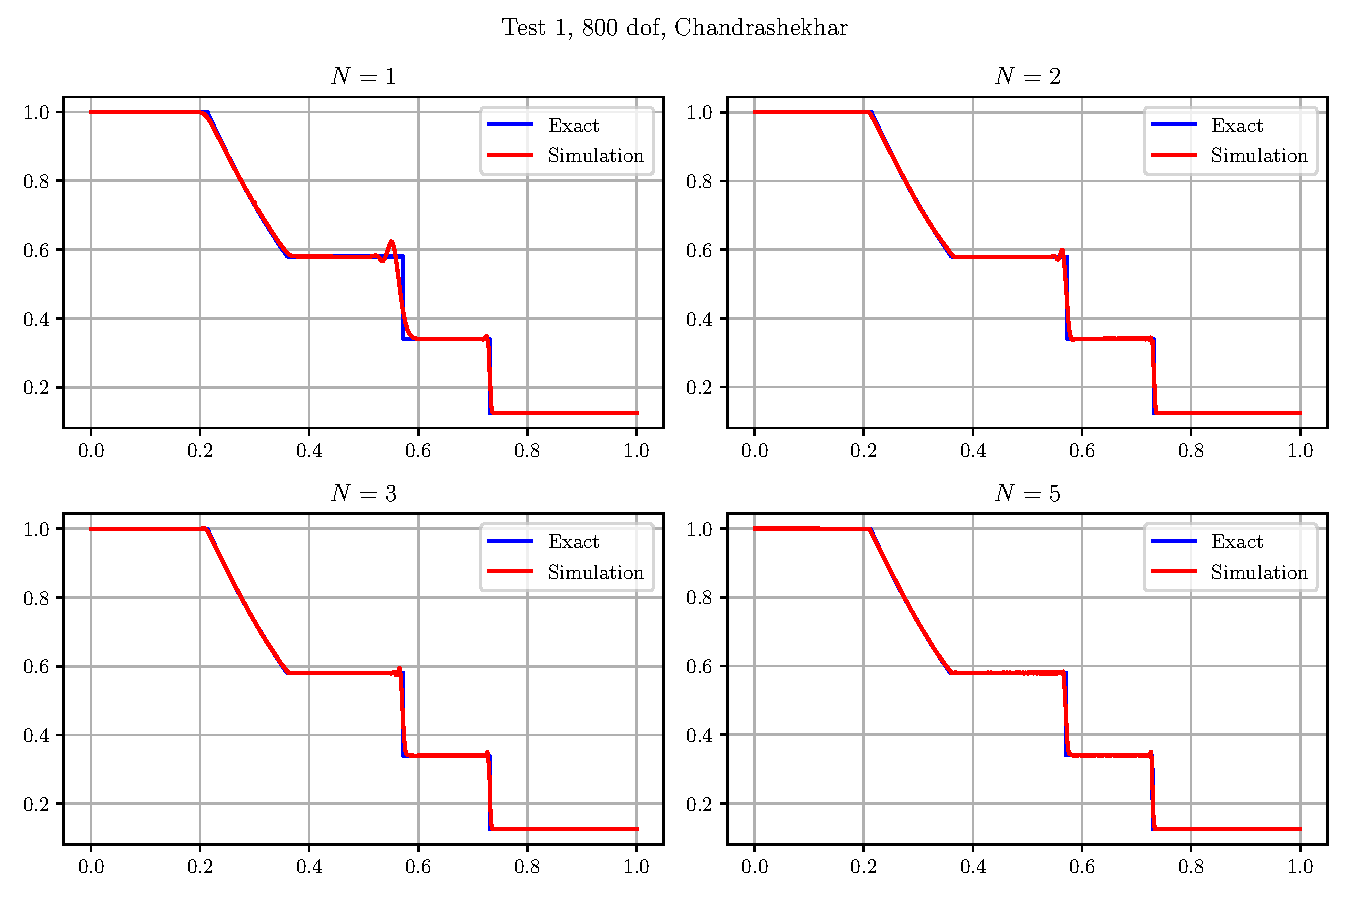
\includegraphics[width=\linewidth]{figures/riemann_1d/test1-1/dof800_12_12_chandrashekhar.pdf}
	\caption{Comparison of density plots for 800 DoFs, Test 1.}
	\label{fig:test1-1_dof800_chandrashekhar}
\end{figure}

\begin{figure}[htbp]
	\centering
	\begin{subfigure}{0.5\linewidth}
		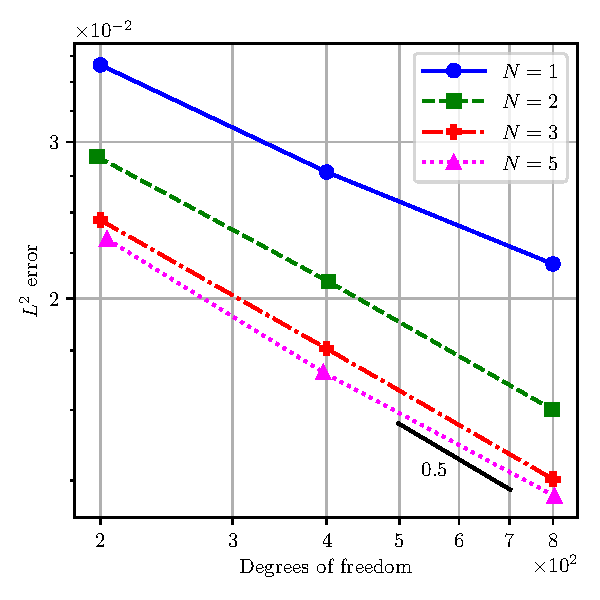
\includegraphics[width=\linewidth]{figures/riemann_1d/test1-1/error_vs_dof_chandrashekhar.pdf}
		\caption{Error vs DoFs.}
		\label{subfig:test1-1_error_vs_dof_chandrashekhar}
	\end{subfigure}%
	\begin{subfigure}{0.5\linewidth}
		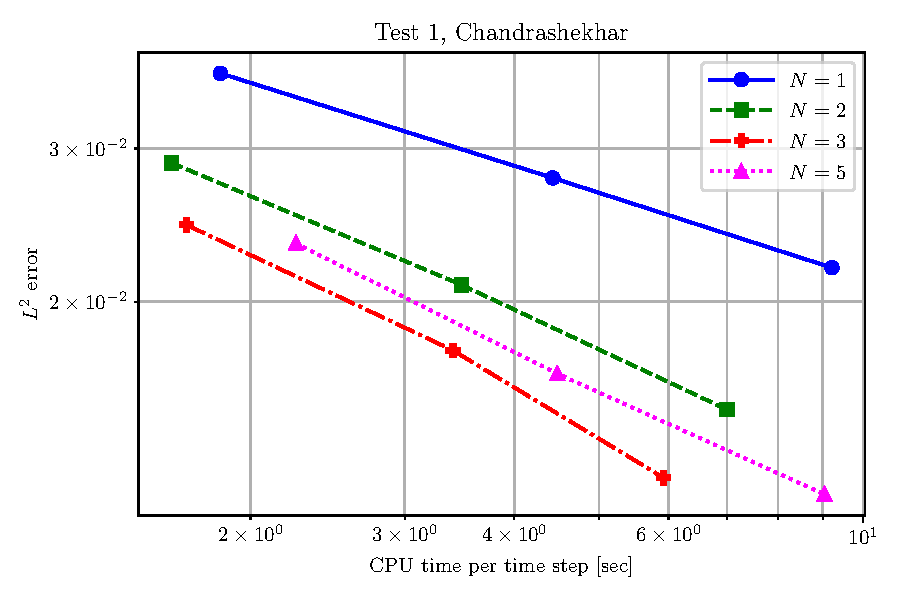
\includegraphics[width=\linewidth]{figures/riemann_1d/test1-1/error_vs_cputime_chandrashekhar.pdf}
		\caption{Error vs CPU time.}
		\label{subfig:test1-1_error_vs_cputime_chandrashekhar}
	\end{subfigure}
	\caption{Statistics for Test 1.}
	\label{fig:test1-1_error_plots_chandrashekhar}
\end{figure}

\subsection{Test 2}
\label[subsection]{subsec:test1-2}

This test consists of two symmetric expansion waves moving away from each other generating very low density and pressure behind their tails and is a relatively difficult case to simulate. It is well known that the behaviour of temperature profile in the low pressure region generated behind the tails of the expansion waves is highly dependent on the particulars of the numerical scheme \cite{toro2009}. \cref{fig:test1-2_dof800_chandrashekhar} shows the comparison of results obtained using 800 DoFs for this case. All results show a temperature peak, failing to faithfully capture the exact variation in the vacuum. However, the extent of discrepancy keeps decreasing with $N$, even though the peak itself does not.

Correspondingly, \cref{subfig:test1-2_error_vs_dof_chandrashekhar} shows that simulations using higher values of $N$ perform more accurately in this case. The error levels keep dropping with $N$: by about a factor of 2 from $N=1$ to $N=5$ for a given DoF resolution. A comparison of the cost shown in \cref{subfig:test1-2_error_vs_cputime_chandrashekhar} tells that $N=5$ simulations also cost much lower than those using $N=2,3$ to get the same error level. Thus in this test case dominated by smooth flow, higher order simulations perform very well and seem to have a clear edge.

\begin{figure}[htbp]
	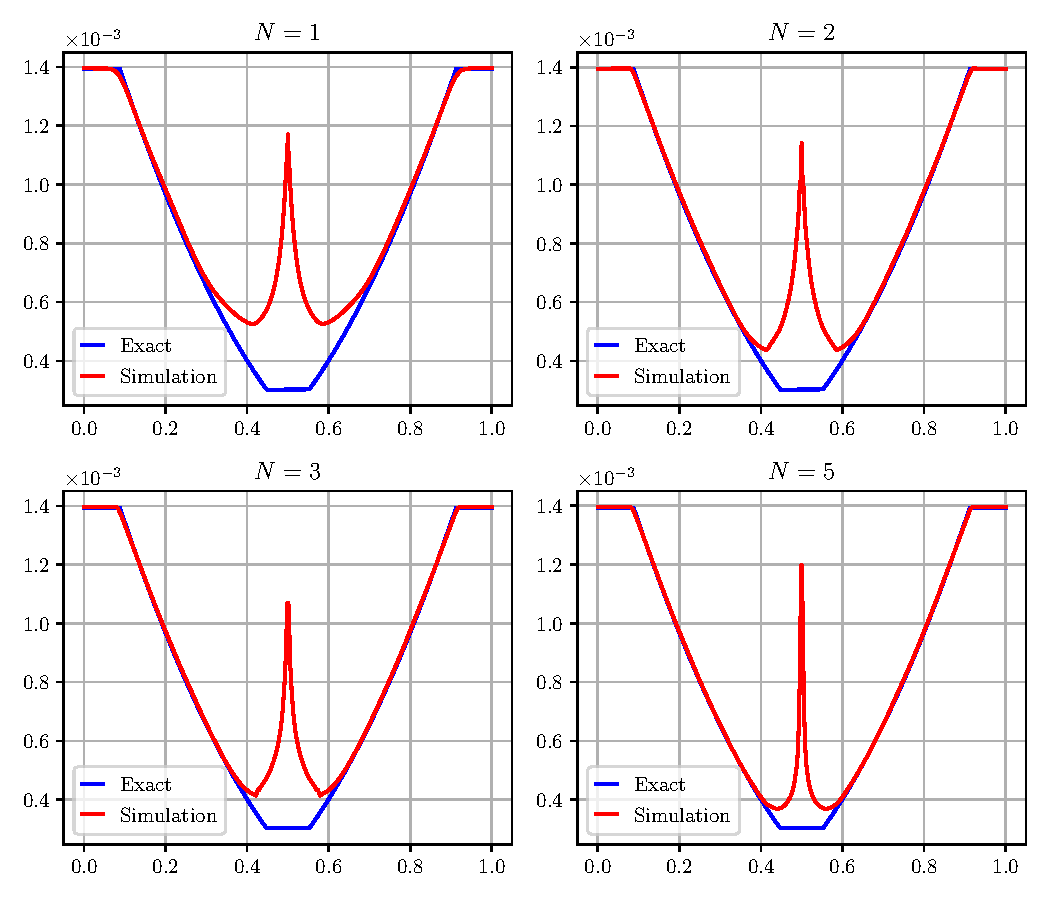
\includegraphics[width=\linewidth]{figures/riemann_1d/test1-2/dof800_12_12_chandrashekhar.pdf}
	\caption{Comparison of temperature plots for 800 DoFs, Test 2.}
	\label{fig:test1-2_dof800_chandrashekhar}
\end{figure}

\begin{figure}[htbp]
	\centering
	\begin{subfigure}{0.5\linewidth}
		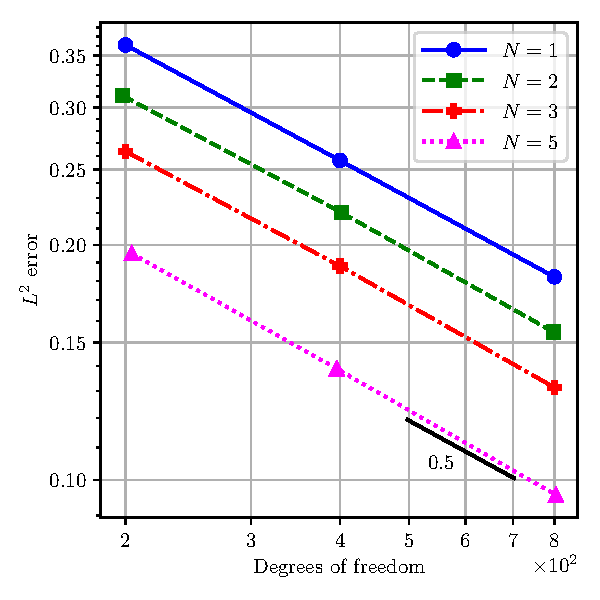
\includegraphics[width=\linewidth]{figures/riemann_1d/test1-2/error_vs_dof_chandrashekhar.pdf}
		\caption{Error vs DoFs.}
		\label{subfig:test1-2_error_vs_dof_chandrashekhar}
	\end{subfigure}%
	\begin{subfigure}{0.5\linewidth}
		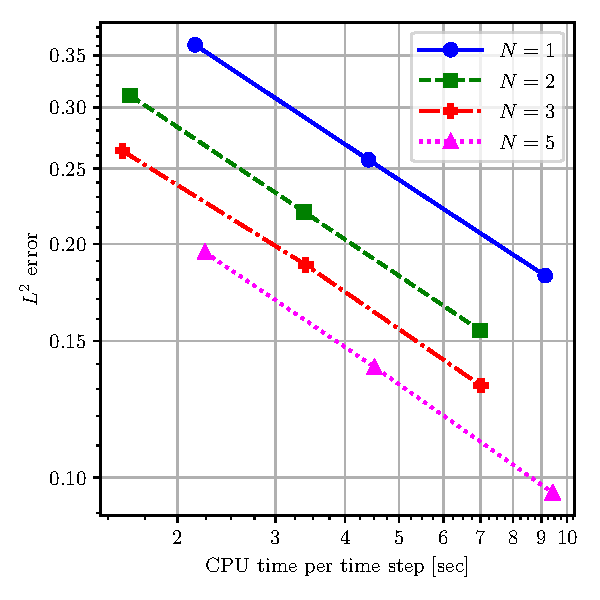
\includegraphics[width=\linewidth]{figures/riemann_1d/test1-2/error_vs_cputime_chandrashekhar.pdf}
		\caption{Error vs CPU time.}
		\label{subfig:test1-2_error_vs_cputime_chandrashekhar}
	\end{subfigure}
	\caption{Statistics for Test 2.}
	\label{fig:test1-2_error_plots_chandrashekhar}
\end{figure}

\subsection{Test 3}
\label[subsection]{subsec:test1-3}

This is again a very severe test case which produces very strong right moving shock (at $x \approx 0.8$) and contact (at $x \approx 0.75$) waves and a left moving expansion wave. The relative speed of the shock and contact waves is very small which makes capturing the high density variation between the contact and shock waves difficult. All results capture the density jump across shock accurately without any diffusion, but produce oscillations before and/or after the shock. While $N=1$ results show a slightly more diffused contact wave, $N=2,3,5$ virtually have an equally good resolution of the same. None of the simulations were able to capture the contact wave as sharply as the shock. The plateau value of density between the very thin region enclosed by contact and shock waves is well-predicted by all simulations.

\cref{subfig:test1-3_error_vs_dof_chandrashekhar} reveals that unlike for Tests 1 and 2, the error levels drop only marginally with increasing $N$ (at a given DoF resolution) for this test. It also shows that there is really no benefit in using $N=5$ here over $N=3$. In fact, it is only more costly than $N=2$ or $N=3$ for a given error level, as is clear from \cref{subfig:test1-3_error_vs_cputime_chandrashekhar}. Considering the visual comparison (shown in \cref{fig:test1-3_dof800_chandrashekhar}) and these error plots together, one can conclude here that $N=3$ is the optimal choice, like in Test 1.

\begin{figure}[htbp]
	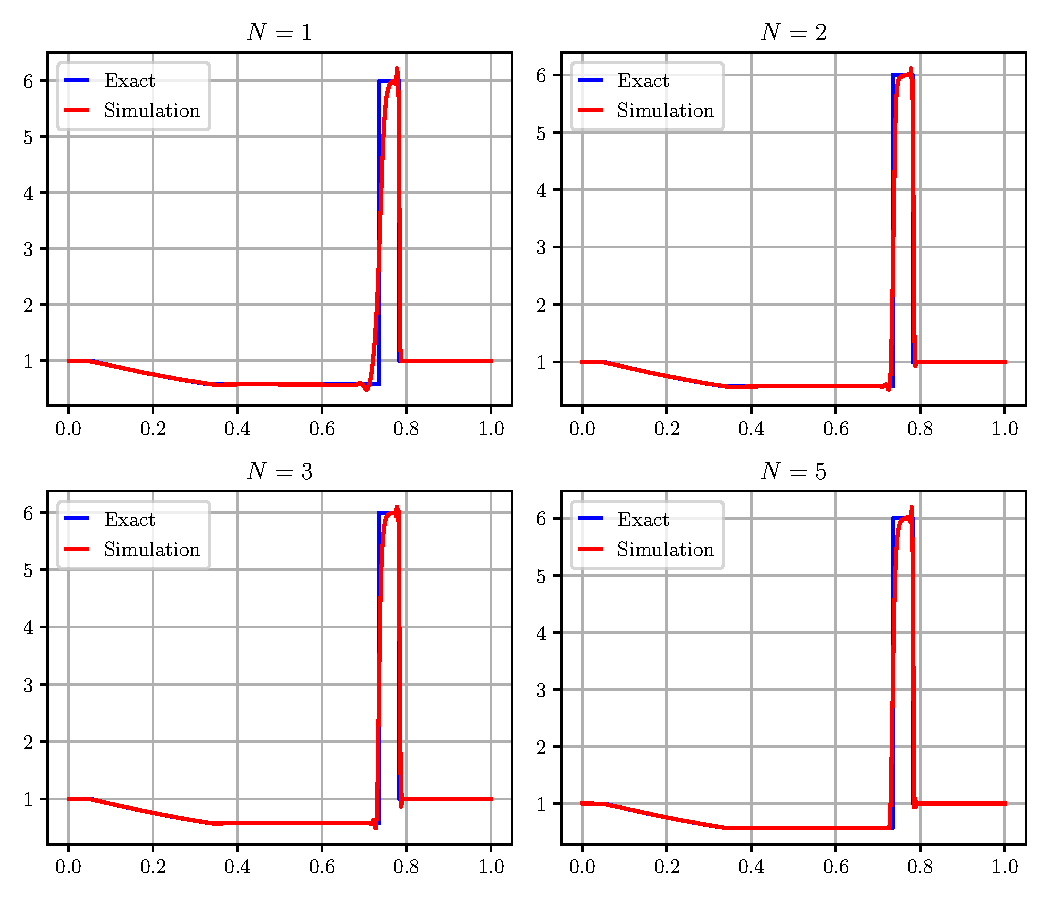
\includegraphics[width=\linewidth]{figures/riemann_1d/test1-3/dof800_12_12_chandrashekhar.pdf}
	\caption{Comparison of density plots for 800 DoFs, Test 3.}
	\label{fig:test1-3_dof800_chandrashekhar}
\end{figure}

\begin{figure}[htbp]
	\centering
	\begin{subfigure}{0.5\linewidth}
		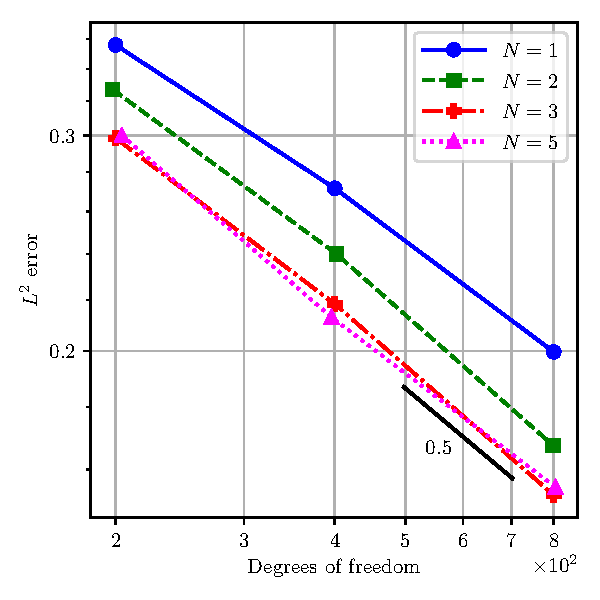
\includegraphics[width=\linewidth]{figures/riemann_1d/test1-3/error_vs_dof_chandrashekhar.pdf}
		\caption{Error vs DoFs.}
		\label{subfig:test1-3_error_vs_dof_chandrashekhar}
	\end{subfigure}%
	\begin{subfigure}{0.5\linewidth}
		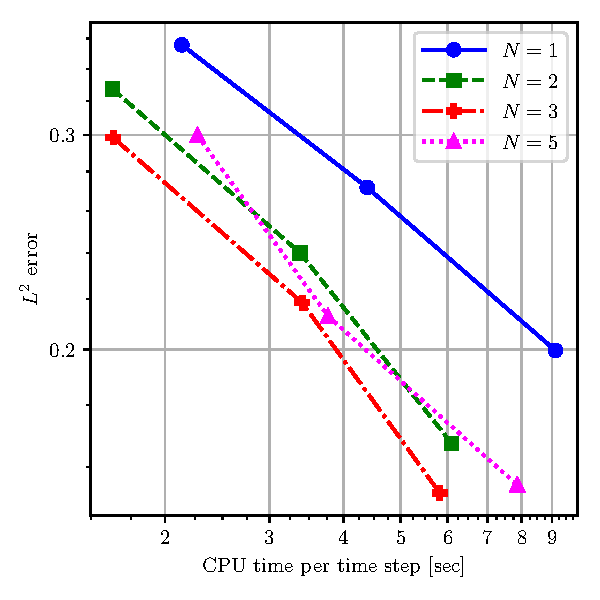
\includegraphics[width=\linewidth]{figures/riemann_1d/test1-3/error_vs_cputime_chandrashekhar.pdf}
		\caption{Error vs CPU time.}
		\label{subfig:test1-3_error_vs_cputime_chandrashekhar}
	\end{subfigure}
	\caption{Statistics for Test 3.}
	\label{fig:test1-3_error_plots_chandrashekhar}
\end{figure}

\subsection{Test 4}
\label[subsection]{subsec:test1-4}

This test case is a strong test case which is generated by impingement of two shocks moving towards each other. The resulting flow contains three discontinuities, all right moving: a slow `left' shock at $x \approx 0.3$, a contact wave at $x \approx 0.6$ and a `right' shock at $x \approx 0.75$. The results obtained with 800 DoFs using $N=1,2,3,5$ are shown in \cref{fig:test1-4_dof800_chandrashekhar}. All simulations capture the left shock sharply and accurately. While the right shock is also sharply resolved, oscillations around the shock are also produced. The resolution of contact wave is almost equally sharp for $N=2,3,5$, while $N=1$ diffuses it slightly more. The most noticeable difference between this test and the previous ones is the presence of significant oscillations in the regions between waves for $N=2,3,5$. Numerical methods are known to produce low frequency oscillations in this test \cite{toro2009,liskaWendroff2003}. The result with $N=3$ seems to have the lowest oscillation level among the three.

Correspondingly, \cref{subfig:test1-4_error_vs_dof_chandrashekhar} reveals that there is hardly any difference made by increasing $N$ beyond 2 for this case. A look at \cref{subfig:test1-4_error_vs_cputime_chandrashekhar} also provides the same conclusion, only that $N=5$ costs higher to give the same error level. While $N=2$ and $N=3$ seem to perform equally well in terms of error and cost, the visual comparison shown in \cref{fig:test1-4_dof800_chandrashekhar}, except for the higher overshoot near the right shock, may lead to concluding in favour of $N=3$ in this case.

\begin{figure}[htbp]
	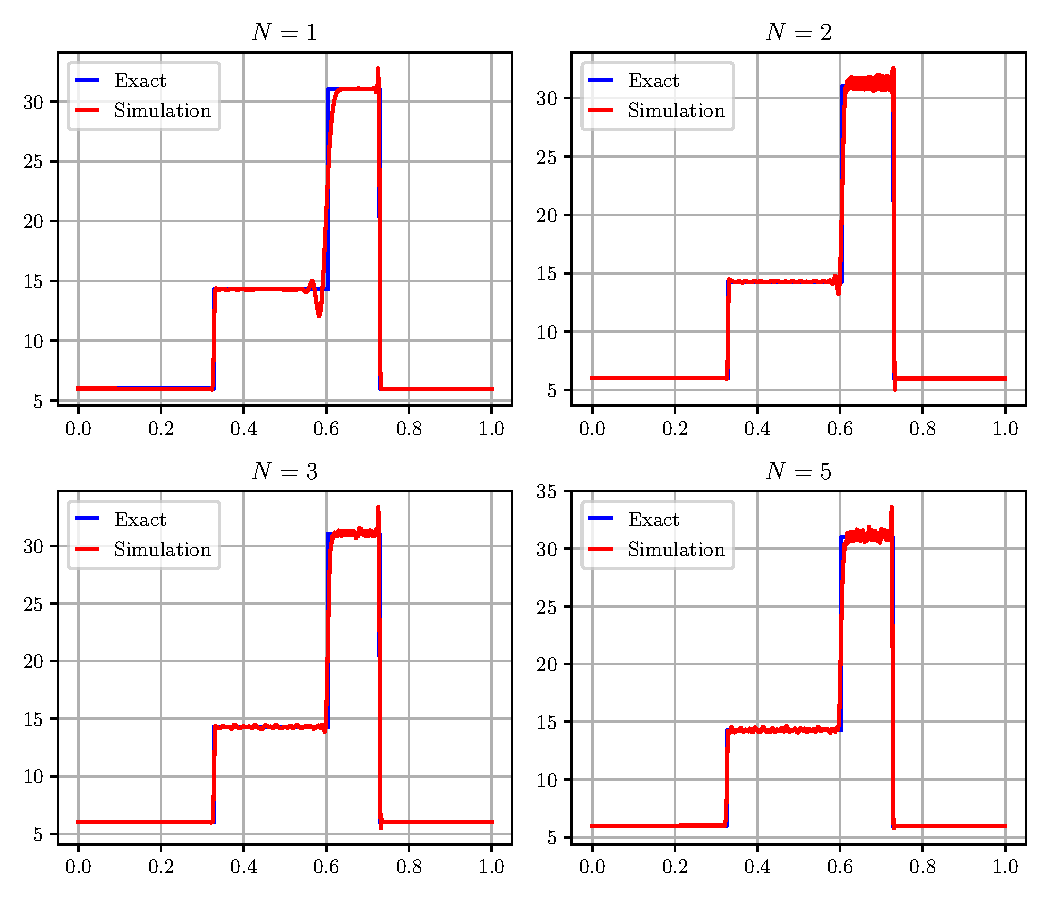
\includegraphics[width=\linewidth]{figures/riemann_1d/test1-4/dof800_12_12_chandrashekhar.pdf}
	\caption{Comparison of density plots for 800 DoFs, Test 4.}
	\label{fig:test1-4_dof800_chandrashekhar}
\end{figure}

\begin{figure}[htbp]
	\centering
	\begin{subfigure}{0.5\linewidth}
		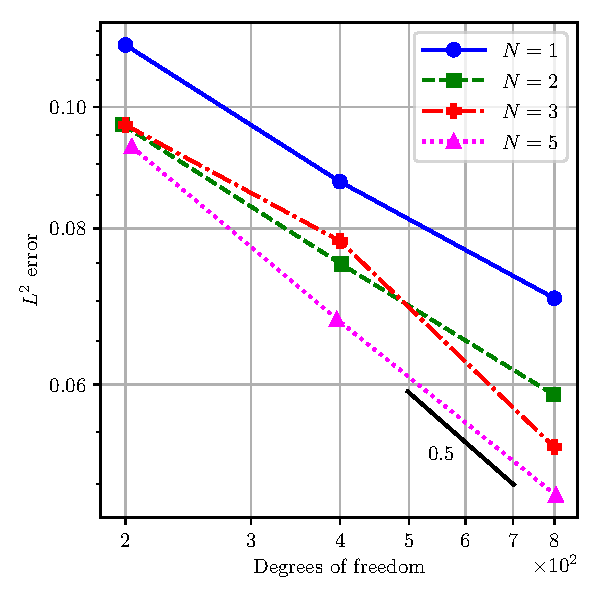
\includegraphics[width=\linewidth]{figures/riemann_1d/test1-4/error_vs_dof_chandrashekhar.pdf}
		\caption{Error vs DoFs.}
		\label{subfig:test1-4_error_vs_dof_chandrashekhar}
	\end{subfigure}%
	\begin{subfigure}{0.5\linewidth}
		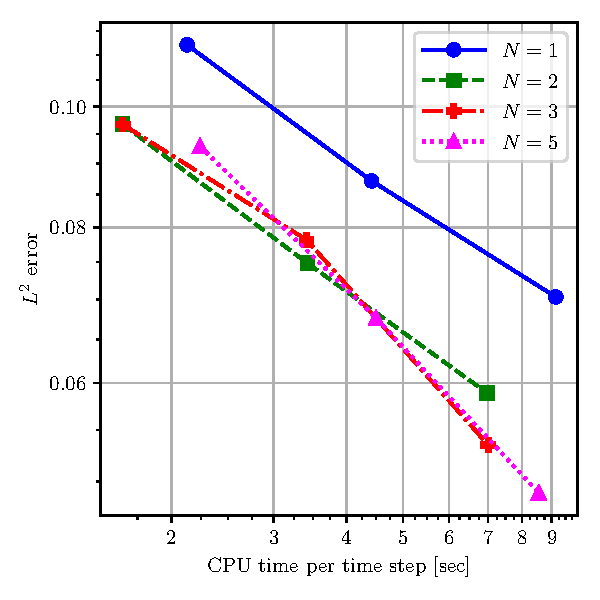
\includegraphics[width=\linewidth]{figures/riemann_1d/test1-4/error_vs_cputime_chandrashekhar.pdf}
		\caption{Error vs CPU time.}
		\label{subfig:test1-4_error_vs_cputime_chandrashekhar}
	\end{subfigure}
	\caption{Statistics for Test 4.}
	\label{fig:test1-4_error_plots_chandrashekhar}
\end{figure}

\subsection{Test 5}
\label[subsection]{subsec:test1-5}

This test is a variation of Test 3 (\cref{subsec:test1-3}) where a background velocity is imposed such that the contact wave becomes stationary. The resulting wave structure thus has two slowly moving waves: a slow right-moving shock (at $x \approx 8.25$) and the stationary contact (at $x=0.8$), in addition to a left-moving expansion. \cref{fig:test1-5_dof800_chandrashekhar} shows the results obtained with 800 DoFs using $N=1,2,3,5$. All simulations achieve sharp resolution of the shock, although, with overshoot and/or undershoot. Like in Tests 3 and 4, $N=2,3,5$ have an equally good resolution of the stationary contact, while $N=1$ has it slightly more diffused. All high order simulations produce oscillations in the region between contact and shock waves, similar to those seen in Test 4. Unlike in Test 4, all high order simulations have produced oscillations of equal magnitudes in this case.

The behaviour of error in this case, shown in \cref{subfig:test1-5_error_vs_dof_chandrashekhar} is also similar to that in Test 4 (\cref{subfig:test1-4_error_vs_dof_chandrashekhar}). There is no remarkable drop in error for a given DoF resolution as $N$ is increased beyond 2. \cref{subfig:test1-5_error_vs_cputime_chandrashekhar} shows that $N=2$ and $N=3$ cost about the same while producing very similar error levels, while $N=5$ costs higher to only produce a small drop in error. Considering the visual comparison of results (\cref{fig:test1-5_dof800_chandrashekhar}), one may conclude that $N=2$ is the optimal choice for this case.

\begin{figure}[htbp]
	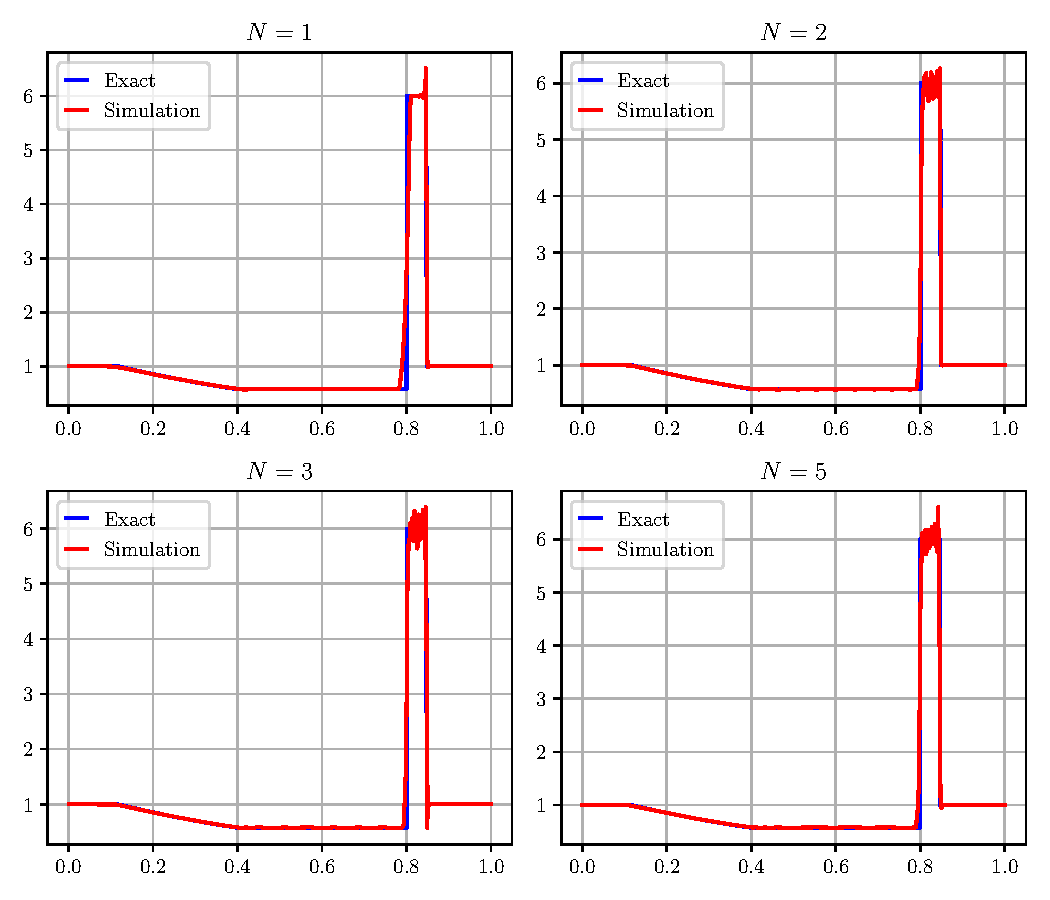
\includegraphics[width=\linewidth]{figures/riemann_1d/test1-5/dof800_12_12_chandrashekhar.pdf}
	\caption{Comparison of density plots for 800 DoFs, Test 5.}
	\label{fig:test1-5_dof800_chandrashekhar}
\end{figure}

\begin{figure}[htbp]
	\centering
	\begin{subfigure}{0.5\linewidth}
		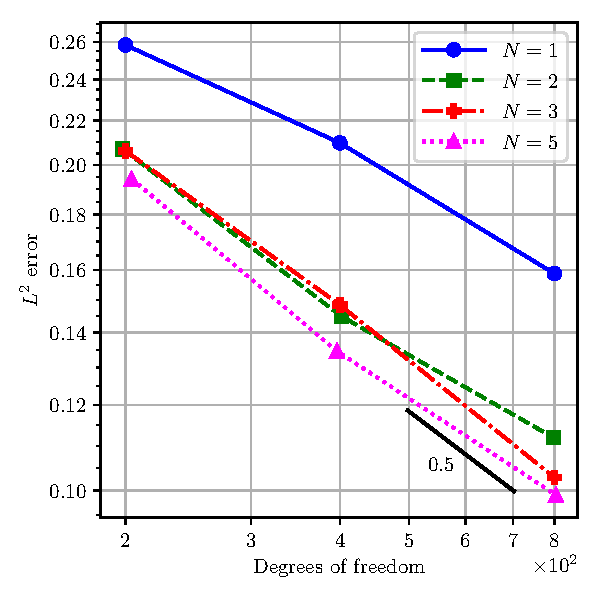
\includegraphics[width=\linewidth]{figures/riemann_1d/test1-5/error_vs_dof_chandrashekhar.pdf}
		\caption{Error vs DoFs.}
		\label{subfig:test1-5_error_vs_dof_chandrashekhar}
	\end{subfigure}%
	\begin{subfigure}{0.5\linewidth}
		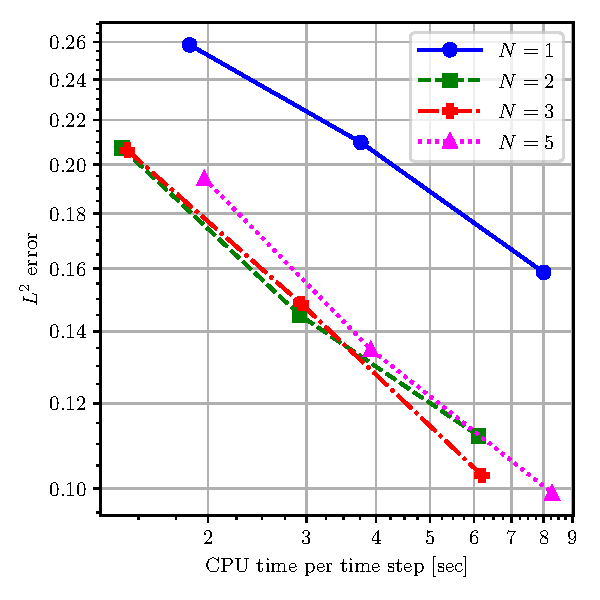
\includegraphics[width=\linewidth]{figures/riemann_1d/test1-5/error_vs_cputime_chandrashekhar.pdf}
		\caption{Error vs CPU time.}
		\label{subfig:test1-5_error_vs_cputime_chandrashekhar}
	\end{subfigure}
	\caption{Statistics for Test 5.}
	\label{fig:test1-5_error_plots_chandrashekhar}
\end{figure}



\section{Two-dimensional test results}
\label{sec:2d_tests}

\subsection{Forward step in a Mach 3 wind tunnel}
\label[subsection]{subsec:forward_facing_step}

This test case proposed by \citear{woodwardColella1984} is a commonly used as a 2d validation test case. The domain $\{[0,3] \times [0,1]\} \setminus \{[0.6,3] \times [0,0.2]\}$ contains a step of height $0.2$, at $x=0.6$ in a wind tunnel of length $3$. The height of the wind tunnel is $1$. The domain is initialised with Mach 3 freestream conditions: $p=1$, $\rho=\gamma$ and $u=3$. A bow shock is generated due to the step, which undergoes multiple reflections from the top and the bottom walls. The first reflection from the top wall is a Mach reflection. The left boundary is imposed with an inflow at freestream conditions, while the right boundary has supersonic outflow. All other boundaries are considered as walls. Although the end time is $t=4$ for this case, simulation results will be compared at $t=3$.

For this case, the meshes for simulations using $N=1,2,3,5$ are generated to give a nominal grid of size $\Delta x = \Delta y \approx (N+1)/80$. Further, the mesh is stretched around the corner to give a cell size 4 times smaller than the nominal size. As a sample, the mesh used for $N=5$ simulation is shown in \cref{fig:forward_facing_step_mesh_N5}. In the $z$ direction, $\lcm \{(N+1) \mid N=1,2,3,5\}$ DoFs are used. \cref{tab:forward_facing_step_mesh_cpu} shows the final mesh size in terms of the number of DoFs for each of the 4 cases.

\cref{fig:forward_facing_step_results} shows the simulation results at time $t=3$. All simulations show a Mach stem at the shock reflection on the bottom wall. This is a numerical artefact which is generated due to entropy production in the expansion wave around corner. It can be seen that the size of this stem reduces as $N$ is increased. Results with $N=2,3$ show carbuncle oscillations in the primary bow shock front. The result with $N=5$ shows some oscillations in the primary shock reflection on the top wall, which are not observed in other cases. All the shocks seem to get slightly more sharper as $N$ is increased. The contact wave generated due to the reflection of primary shock on the top wall is more sharply resolved with $N=2,5$. In conclusion, it can be said in this case that high order schemes introduce less entropy production around the corner expansion, although they display the carbuncle phenomenon. Considering the CPU time per time step{---}shown in \cref{tab:forward_facing_step_mesh_cpu}{---} along with the visual results, $N=2$ seems to perform marginally better here than other cases.

\begin{table}[htbp]
	\centering
	\caption{Mesh details and computational cost per time step for forward step case.}
	\label{tab:forward_facing_step_mesh_cpu}
	\begin{tabular}{S[table-format=1.0, table-text-alignment=left] S[table-format=5.0, table-text-alignment=left] S[table-format=6.0, table-text-alignment=left] S[table-format=2.2, table-text-alignment=left]}
		\toprule
		{$N$} & {Number of cells} & {Number of DoFs} & {CPU time per time step (sec)} \\
		\midrule
		1 & 24192 & 193536 & 16.24 \\
		2 & 7624 & 205848 & 12.78 \\
		3 & 3024 & 193536 & 12.63 \\
		5 & 978 & 211248 & 16.94 \\
		\bottomrule
	\end{tabular}
\end{table}

\begin{figure}[htbp]
	\centering
	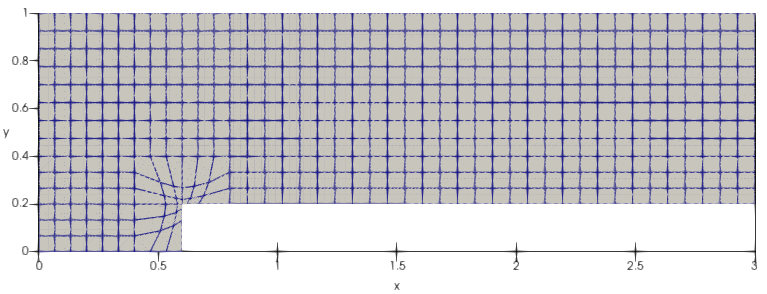
\includegraphics[width=0.8\linewidth]{figures/forward_facing_step/mesh_N5}
	\caption{Mesh used for $N=5$ simulation of the forward step case.}
	\label{fig:forward_facing_step_mesh_N5}
\end{figure}

\begin{figure}[htbp]
	\centering
	\begin{subfigure}{0.5\linewidth}
		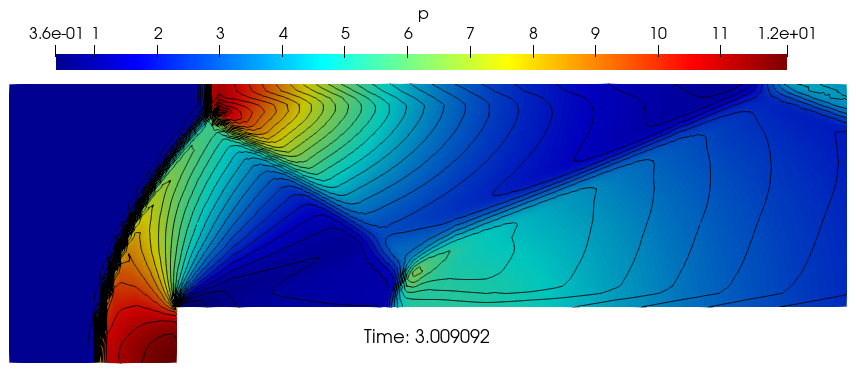
\includegraphics[width=\linewidth]{figures/forward_facing_step/res_40_N1_chandrashekhar_t3}
		\caption{$N=1$.}
		\label{subfig:forward_facing_step_result_N1}
	\end{subfigure}%
	\begin{subfigure}{0.5\linewidth}
		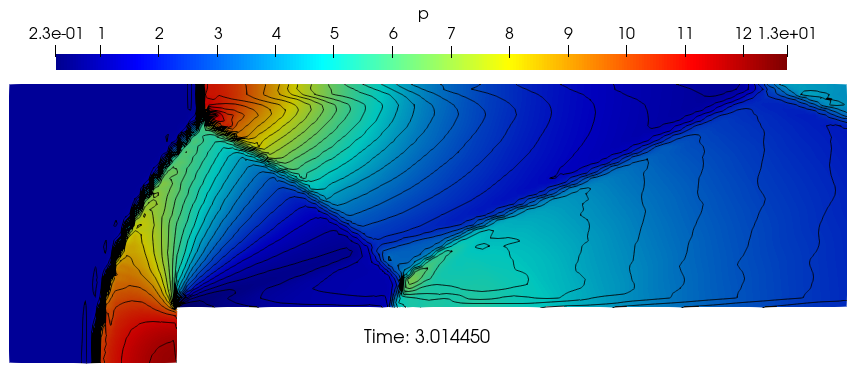
\includegraphics[width=\linewidth]{figures/forward_facing_step/res_40_N2_chandrashekhar_t3}
		\caption{$N=2$.}
		\label{subfig:forward_facing_step_result_N2}
	\end{subfigure}\\
	\begin{subfigure}{0.5\linewidth}
		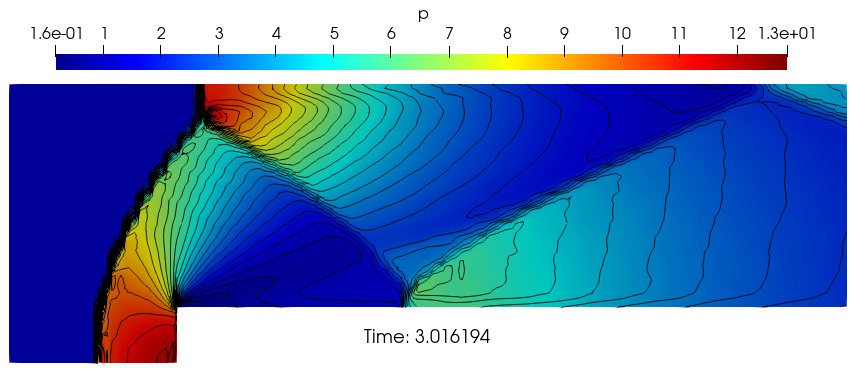
\includegraphics[width=\linewidth]{figures/forward_facing_step/res_40_N3_chandrashekhar_t3}
		\caption{$N=3$.}
		\label{subfig:forward_facing_step_result_N3}
	\end{subfigure}%
	\begin{subfigure}{0.5\linewidth}
		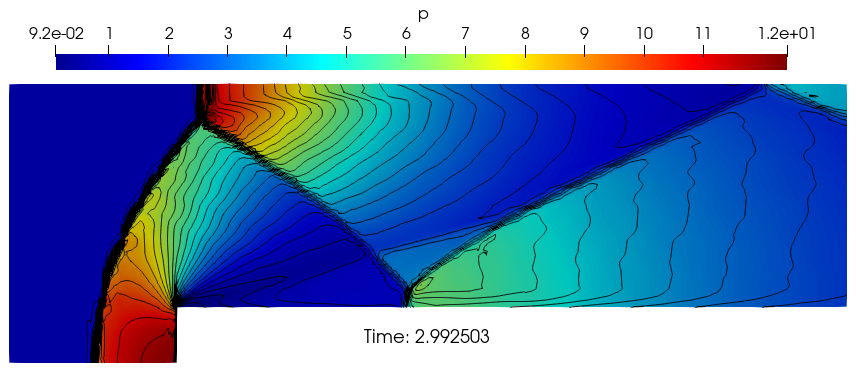
\includegraphics[width=\linewidth]{figures/forward_facing_step/res_40_N5_chandrashekhar_t3}
		\caption{$N=5$.}
		\label{subfig:forward_facing_step_result_N5}
	\end{subfigure}\\
	\begin{subfigure}{0.5\linewidth}
		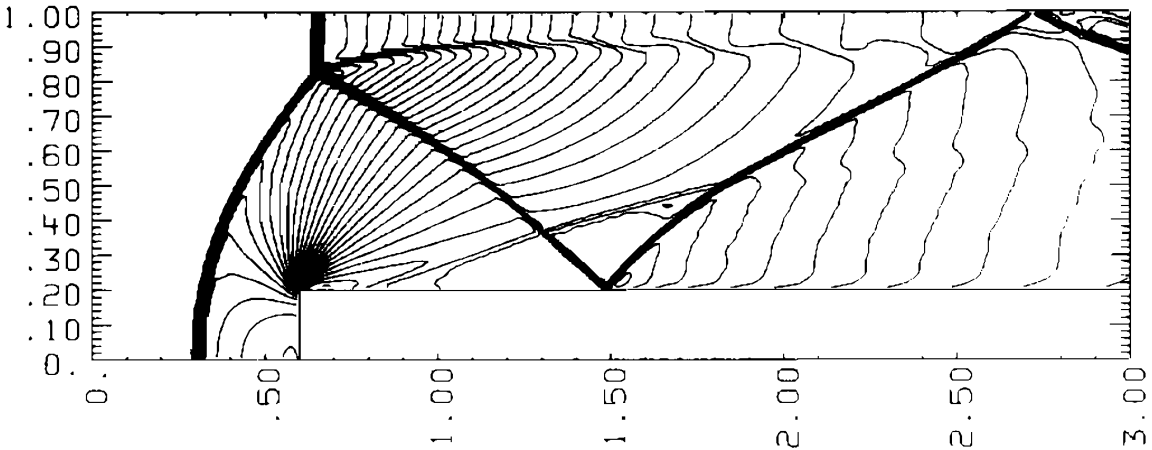
\includegraphics[width=\linewidth]{figures/forward_facing_step/woodward_rho_contour_3}
		\caption{Reference solution.}
		\label{subfig:forward_facing_step_woodward_rho_contour_3}
	\end{subfigure}
	\caption{Results for forward step case at simulation time $t \approx 3$. In all plots, the 30 density contours are shown along with a pressure surface plot. The minimum and maximum values for density contours are variable across the cases. The reference solution by \citear{woodwardColella1984} plots 30 density contours using PPMLR scheme and an `entropy fix' at the corner, on a mesh with size $\Delta x = \Delta y = 1/80$.}
	\label{fig:forward_facing_step_results}
\end{figure}

\subsection{Double Mach reflection}
\label[subsection]{subsec:dmr}

This test case, again proposed by \citear{woodwardColella1984}, is concerned with the reflection of a Mach 10 shock hitting a ramp angled \SI{30}{\degree}. Both the incident and the reflected shocks undergo a Mach reflection producing a complex wave structure. Following \citear{kemm2016}, the problem is setup on a domain of size $[0,4] \times [0,2]$ with the incident shock initially inclined \SI{60}{\degree} to the wall, which is one part $[1/6,4]$ of the bottom boundary. The other part of the bottom boundary $[0,1/6]$ along with the left side is given post-shock inflow conditions. The top and the right boundaries are given exact boundary conditions to capture the motion of the shock. Pre-shock conditions are $p=1$, $\rho=\gamma$ and $u=0=v$, and the post-shock conditions are calculated using normal shock relations.

The meshes used in this case are designed to have $\Delta x = \Delta y \approx (N+1)/120$ for $N=1,2,3,5$, along with $\lcm \{ (N+1) \mid N=1,2,3,5 \} = 12$ DoFs in the $z$ direction. \cref{tab:dmr_mesh_cpu} shows the total number of DoFs in the mesh for different values of $N$.

\cref{fig:dmr_results} shows the results obtained with $N=1,2,3,5$ at end time $t=0.2$. It is immediately clear that all high order simulations capture the bending of the slip line emanating from the first triple point much better compared to $N=1$. They also capture the shock emanating from the secondary triple point better. While $N=5$ gives the sharpest resolution of the primary shock structures (namely incident shock, primary Mach stem and reflected shock along with its Mach stem), the other secondary structures are equally well resolved with $N=2,3,5$. Considering the CPU cost required by each of the schemes (shown in \cref{tab:dmr_mesh_cpu}) along with the visual results, one can conclude that $N=3$ is the best performer in this case.

\begin{table}[htbp]
    \centering
    \caption{Mesh details and computational cost per time step for the double Mach reflection case.}
    \label{tab:dmr_mesh_cpu}
    \begin{tabular}{S[table-format=1.0, table-text-alignment=left] S[table-format=6.0, table-text-alignment=left] S[table-format=7.0, table-text-alignment=left] S[table-format=3.2, table-text-alignment=left]}
        \toprule
        {$N$} & {Number of cells} & {Number of DoFs} & {CPU time per time step (sec)} \\
        \midrule
        1 & 172800 & 1382400 & 131.3 \\
        2 & 51520 & 1391040 & 97.3 \\
        3 & 21600 & 1382400 & 92.93 \\
        5 & 6480 & 1399680 & 124.1 \\
        \bottomrule
    \end{tabular}
\end{table}

\begin{figure}[htbp]
	\centering
	\begin{subfigure}{0.5\linewidth}
		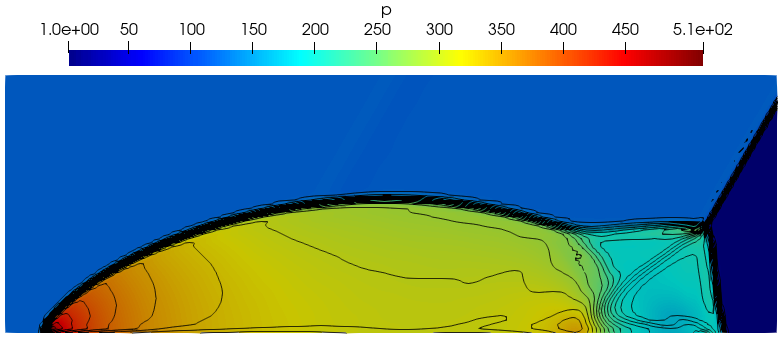
\includegraphics[width=\linewidth]{figures/dmr/res_60_N1_chandrashekhar}
		\caption{$N=1$.}
		\label{subfig:dmr_result_N1}
	\end{subfigure}%
	\begin{subfigure}{0.5\linewidth}
		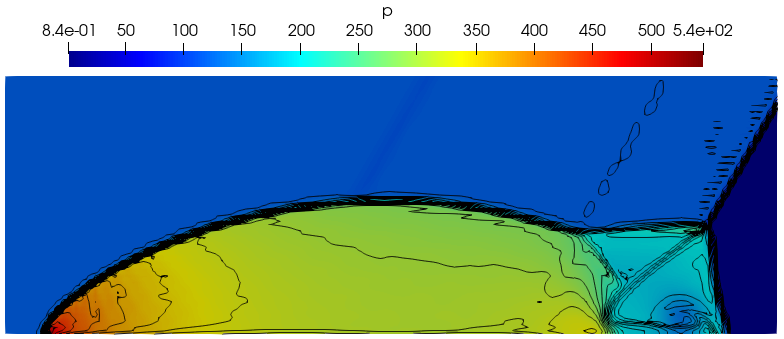
\includegraphics[width=\linewidth]{figures/dmr/res_60_N2_chandrashekhar}
		\caption{$N=2$.}
		\label{subfig:dmr_result_N2}
	\end{subfigure}\\
	\begin{subfigure}{0.5\linewidth}
		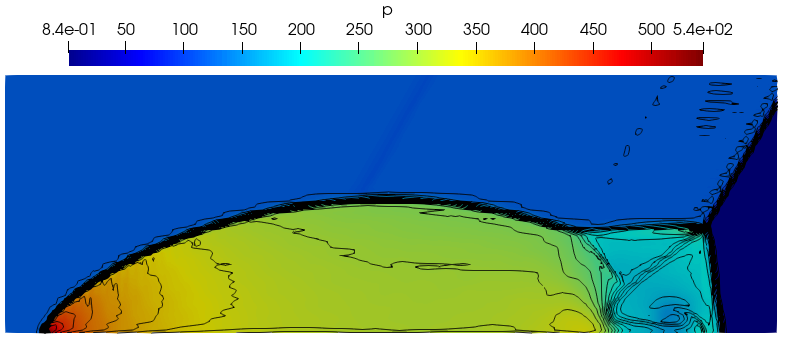
\includegraphics[width=\linewidth]{figures/dmr/res_60_N3_chandrashekhar}
		\caption{$N=3$.}
		\label{subfig:dmr_result_N3}
	\end{subfigure}%
	\begin{subfigure}{0.5\linewidth}
		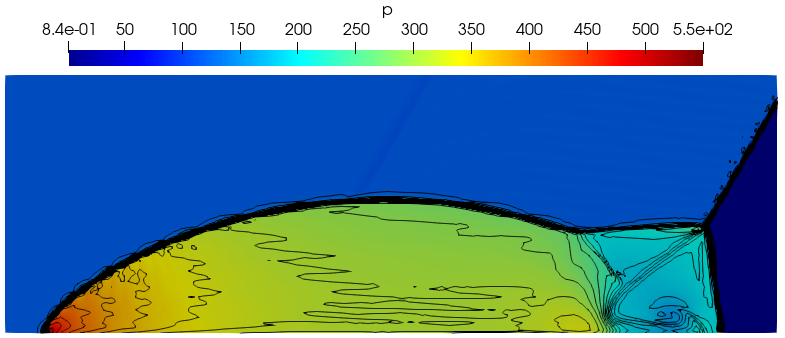
\includegraphics[width=\linewidth]{figures/dmr/res_60_N5_chandrashekhar}
		\caption{$N=5$.}
		\label{subfig:dmr_result_N5}
	\end{subfigure}\\
	\begin{subfigure}{0.5\linewidth}
		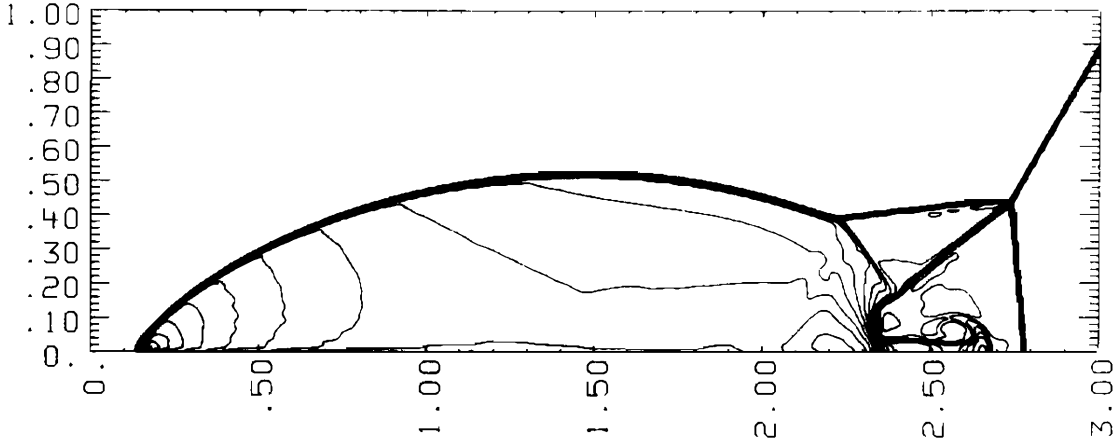
\includegraphics[width=\linewidth]{figures/dmr/woodward_rho_contour}
		\caption{Reference solution.}
		\label{subfig:dmr_woodward_rho_contour}
	\end{subfigure}
	\caption{Results for double Mach reflection case. All figures show pressure surface plot with 30 density contours. The contour levels vary across the cases. The reference solution is by \citear{woodwardColella1984} using PPMDE method on a grid of size $\Delta x = \Delta y = 1/120$.}
    \label{fig:dmr_results}
\end{figure}

\printbibliography
\end{document}